\blandscape
\begin{figure}[H]
\centering
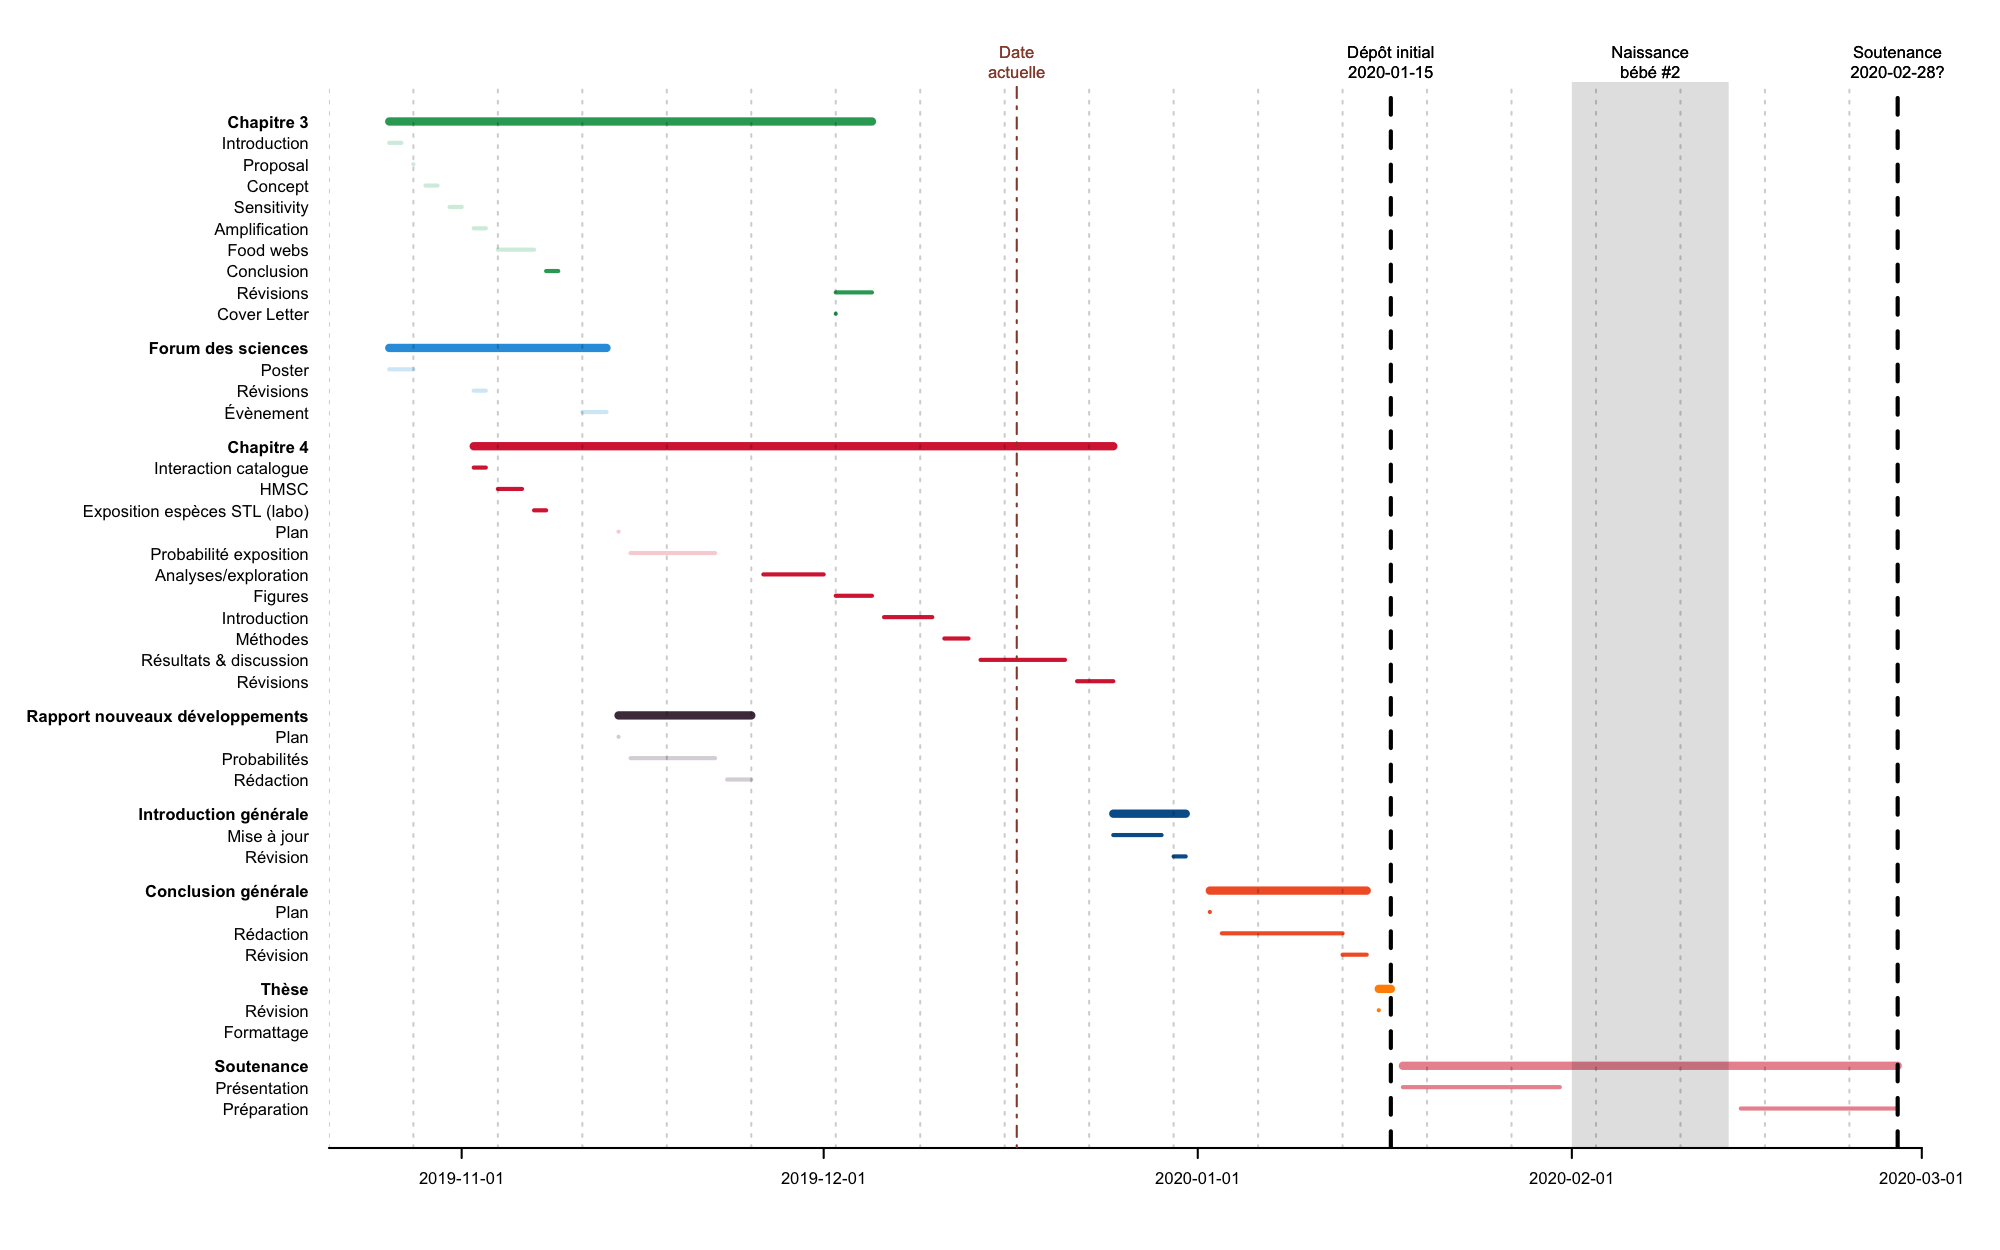
\includegraphics[width=\columnwidth]{./timeline.png}
\label{timeline}
\end{figure}
\elandscape
\newpage

\hypertarget{checklist}{%
\section{Checklist}\label{checklist}}

\begin{itemize}
\tightlist
\item[$\square$]
  Composition jury
\item[$\square$]
  Dédicace(?)
\item[$\square$]
  Remerciements
\item[$\square$]
  Avant-propos
\item[$\square$]
  Résumé de la thèse (fr)
\item[$\square$]
  Résumé de la thèse (en)
\item[$\square$]
  Liste des abbréviations(?)
\item[$\square$]
  Introduction générale
\item[$\square$]
  Chapitre 1: Ecology Letters paper
\item[$\square$]
  Chapitre 2: Frontiers in Marine Sciences - Drivers
\item[$\square$]
  Chapitre 3: iEat
\item[$\square$]
  Chapitre 4: Cumulative impacts on food webs
\item[$\square$]
  Conclusion générale
\item[$\square$]
  Annexe 1: Supplementary information chapitre 1
\item[$\square$]
  Annexe 2: Supplementary information chapitre 2
\item[$\square$]
  Annexe 3: Supplementary information chapitre 3
\item[$\square$]
  Annexe 4: Supplementary information chapitre 4
\item[$\square$]
  References
\end{itemize}

\hypertarget{introduction-guxe9nuxe9rale}{%
\subsection{Introduction générale}\label{introduction-guxe9nuxe9rale}}

\begin{itemize}
\tightlist
\item[$\square$]
  Réviser introduction générale
\item[$\square$]
  Mettre à jour avec la littérature récente
\item[$\square$]
  Mettre à jour les objectifs de la thèse
\end{itemize}

\hypertarget{chapitre-1}{%
\subsection{Chapitre 1}\label{chapitre-1}}

\begin{itemize}
\tightlist
\item[$\square$]
  Contexte scientifique (Thèse)
\item[$\square$]
  Publication associée (Thèse)
\item[$\square$]
  Traduction du résumé de l'article publié (Thèse)
\item[$\square$]
  Proposal letter Ecology Letters - Ideas and Perspectives
\item[$\square$]
  Cover letter and novelty statement
\item[$\boxtimes$]
  Conflict of interest statement
\item[$\square$]
  Statement of authorship
\item[$\square$]
  Data accessibility statement
\item[$\square$]
  Reviewers
\item[$\square$]
  Keywords
\item[$\square$]
  Abstract
\item[$\square$]
  Introduction
\item[$\square$]
  Of food webs and multiple disturbances (concept)
\item[$\square$]
  Simulations
\item[$\square$]
  Sensitivity
\item[$\square$]
  Amplification
\item[$\square$]
  Food web sensitivity \& amplification
\item[$\square$]
  Conclusions
\item[$\square$]
  Acknowledgements
\item[$\square$]
  References
\item[$\square$]
  Figure 1 - Concept
\item[$\square$]
  Figure 2 - Sensitivity
\item[$\square$]
  Figure 3 - Amplification
\item[$\square$]
  Figure 4 - Food web scores table
\item[$\square$]
  Figure 5 - Topological \textasciitilde{} Realised scores
\item[$\square$]
  Figure 6 - Scores \textasciitilde{} Trophic level \& degree
\item[$\square$]
  Table S1 - Systems of equations
\item[$\square$]
  Article formatting
\end{itemize}

\hypertarget{chapitre-2}{%
\subsection{Chapitre 2}\label{chapitre-2}}

\begin{itemize}
\tightlist
\item[$\square$]
  Retranscrire article
\item[$\square$]
  Contexte scientifique (Thèse)
\item[$\square$]
  Publication associée (Thèse)
\item[$\square$]
  Traduction du résumé de l'article publié (Thèse)
\item[$\boxtimes$]
  Références
\item[$\boxtimes$]
  Table
\item[$\boxtimes$]
  Figures
\item[$\boxtimes$]
  Box
\item[$\square$]
  keywords
\end{itemize}

\hypertarget{chapitre-3}{%
\subsection{Chapitre 3}\label{chapitre-3}}

\begin{itemize}
\tightlist
\item[$\square$]
  Retranscrire article
\item[$\square$]
  Contexte scientifique (Thèse)
\item[$\square$]
  Publication associée (Thèse)
\item[$\square$]
  Traduction du résumé de l'article publié (Thèse)
\item[$\square$]
  Références
\item[$\square$]
  keywords
\item[$\square$]
  Format table in appendice
\end{itemize}

\hypertarget{chapitre-4}{%
\subsection{Chapitre 4}\label{chapitre-4}}

\begin{itemize}
\tightlist
\item[$\square$]
  Données
\item[$\square$]
  Catalogue interactions
\item[$\square$]
  HMSC
\item[$\square$]
  Probabilité d'exposition
\item[$\square$]
  Rapport nouveaux développements en océanographie
\item[$\square$]
  Plan article
\item[$\square$]
  Article de soumission
\end{itemize}

\hypertarget{conclusion-guxe9nuxe9rale}{%
\subsection{Conclusion générale}\label{conclusion-guxe9nuxe9rale}}

\begin{itemize}
\tightlist
\item[$\square$]
  Plan conclusion générale
\item[$\square$]
  Brainstorm
\end{itemize}
